\documentclass[conference,letterpaper]{IEEEtran}
\usepackage{cite}
\usepackage{amsmath,amssymb,bm}
\usepackage{graphicx}
\usepackage{booktabs}
\usepackage{multirow}
\usepackage{siunitx}
\usepackage{tikz}
\usepackage{dblfloatfix}
\usepackage{placeins}
\flushbottom

\usetikzlibrary{arrows.meta,positioning,fit,calc}

\graphicspath{{figures_twc_generated/}{../figures_twc_generated/}{../../figures_twc_generated/}}


\setlength{\textfloatsep}{8pt plus 2pt minus 2pt}
\setlength{\dbltextfloatsep}{8pt plus 2pt minus 2pt}
\setlength{\floatsep}{6pt plus 2pt minus 2pt}
\setlength{\dblfloatsep}{6pt plus 2pt minus 2pt}
\setlength{\intextsep}{6pt plus 2pt minus 2pt}
\setlength{\abovecaptionskip}{4pt}
\setlength{\belowcaptionskip}{0pt}
\renewcommand{\topfraction}{0.9}
\renewcommand{\textfraction}{0.1}

% --- IEEE GLOBECOM checker layout fixes ---
% The checker measured a 0.166 in gutter and requires >= 0.2 in.
% Use a small safety buffer while minimizing reflow.
\setlength{\columnsep}{0.22in}

% The checker measured a 0.68 in top margin on page 4 and requires >= 0.70 in.
% Move the text block down 0.05 in, and reduce textheight by the same amount
% so the bottom margin is not worsened.
\addtolength{\topmargin}{0.05in}
\addtolength{\textheight}{-0.05in}

% Keep the conference submission free of page numbers/running headers.
\pagestyle{empty}

\sisetup{
	detect-all,
	group-minimum-digits = 3,
	table-number-alignment = center
}

\newcommand{\snr}{E_b/N_0}
\begin{document}
	\title{UPAIR: Universal Prompted Axial In-context Estimator
		for 5G New Radio Uplink}
	\author{
		\IEEEauthorblockN{Ali Fazeli\textsuperscript{*}, Raviraj Adve\textsuperscript{*}, Akram~bin~Sediq\textsuperscript{\dag}, Amr~El-Keyi\textsuperscript{\dag}, and Ahmad Khan\textsuperscript{\dag}}
		\IEEEauthorblockA{\textsuperscript{*}\textit{Dept. of Electrical and Computer Engineering, University of Toronto}, Toronto, Canada}
		\IEEEauthorblockA{\textsuperscript{\dag}\textit{Ericsson Canada}, Ottawa, Canada}
		\IEEEauthorblockA{emails: \{ali.fazeli@, rsadve@ece.\}utoronto.ca, \{akram.bin.sediq, amr.el-keyi, ahmad.a.khan\}@ericsson.com}
	}
	
	\markboth{}%
	{Fazeli \MakeLowercase{\textit{et al.}}: Universal Prompted Axial In-context Estimator for 5G NR Uplink}
	
	\maketitle
	
	\begin{abstract}
		This paper proposes UPAIR (Universal Prompted Axial In-context estimatoR), a prompted channel-estimation front-end for 5G New Radio (NR). The estimator plugs into the standard NR uplink receiver chain, leaving the rest of the chain unchanged. Starting from a least-squares (LS) estimate on the demodulation reference signals (DMRS), UPAIR forms a slot-level prompt that conditions feature-wise linear modulation (FiLM) axial refinement blocks, and outputs a channel estimate together with an uncertainty map consumed by the downstream linear minimum mean-square error (LMMSE) detector.
		We evaluate UPAIR against classical channel estimators in three scenarios: a clean reference case, a mild phase-distortion case, and a DMRS-rich mild phase-distortion case.
		Across these scenarios at BLER of $10^{-2}$, UPAIR achieves gains of $0.80$~dB and $1.18$~dB compared to the strongest classical baseline in the clean and mild phase-distortion settings, respectively, while remaining only about $0.55$~dB from the perfect-CSI benchmark in both settings. In the DMRS-rich mild phase-distortion setting, UPAIR is essentially tied with the strongest classical baseline. Over the full evaluated SNR grid, UPAIR also yields the lowest channel-estimation error in all three scenarios.
		
	\end{abstract}
	
	%	\vspace{-.5cm}
	\section{Introduction}
	\label{sec:introduction}
	
	
	\IEEEPARstart{R}{eliable} channel estimation remains a central requirement in 5G New Radio (NR) because detection and decoding depends directly on the channel state information (CSI) extracted from the demodulation reference signals (DMRS) defined by the standard~\cite{3gpp38211,3gpp38214}. Classical OFDM studies established techniques that still underlie practical receivers, including single-value decomposition-based linear minimum mean squared error (LMMSE) estimation~\cite{edfors1998}, robust MMSE estimation for dispersive channels~\cite{li1998}, and pilot-aided maximum likelihood and Bayesian MMSE~\cite{morelli2001}.
	
	A related challenge is oscillator impairment: OFDM sensitivity to carrier-frequency offset and Wiener phase noise~\cite{pollet1995}, and the resulting common phase error~\cite{wu2004}, remain relevant whenever the density of pilot symbols is limited and the receiver must interpolate while also tracking phase variations.
	
	Deep learning (DL) has provided an alternative to purely model-based estimation~\cite{oshea2017,qin2019,he2019}, with OFDM-specific studies demonstrating gains in channel estimation and signal detection under distortion~\cite{ye2018}.
	In this direction, axial self-attention factorizes attention along the time and frequency axes, matching the separable structure of OFDM and reducing complexity~\cite{yellapragada2025}, while more recent efforts target standard-compliant deployments, including a neural receiver for 5G NR multi-user MIMO~\cite{cammerer2023} and real-time operation under latency constraints~\cite{wiesmayr2025}.
	
	A recent trend is prompt-based or in-context wireless inference. In~\cite{kunde2025}, transformers were shown to asymptotically achieve optimal in-context estimation for a class of wireless estimation problems. Further   work then extended this idea to decision-feedback symbol detection~\cite{fan2025} and to a multi-task OFDM transformer for channel estimation and symbol detection without task-specific fine-tuning~\cite{kou2025}. Together, these results show that adaptation can come from the current input and context, rather than from retraining during deployment.
	
	In parallel, large-model ideas also began to influence wireless channel processing. Recent examples include LLM-based multi-task wireless processing~\cite{llm4wm2025}, generative pre-training and large-model channel modeling~\cite{wirelessgpt2025,channelgpt2025}, direct use of pre-trained vision models for CSI-related tasks~\cite{lvm4csi2025}, and context-conditioned estimators based on adaptive transformers and feature-wise linear modulation (FiLM)-guided diffusion~\cite{adafortitran2025,mohsin2025}. Overall, these works show that prompting, context conditioning, and large models are relevant not only to broader wireless learning tasks but also to channel estimation itself.
	
	We adopt a practical design constraint: only the channel-estimation front-end of the standard-compliant 5G NR uplink chain is modified, while the downstream detection and decoding remain unchanged. This keeps the receiver standard-compatible and, since the perfect-CSI curve uses the same downstream chain, makes any gap to it a pure channel-estimation gap. The present paper follows this direction and proposes \underline{U}niversal \underline{P}rompted \underline{A}xial \underline{I}n-context estimato\underline{R} (UPAIR{}), a slot-conditioned channel-estimation front-end for 5G NR. Starting from an LS reference, it maps current-slot observations to a feature tensor, forms a slot prompt by demodulation reference signals (DMRS)-masked averaging of the projected features followed by a small multilayer perceptron (MLP), and refines the estimate through FiLM-conditioned axial processing~\cite{film,axial}. 
	
	Numerical results show UPAIR outperforms practical baselines and approaches perfect-CSI within a standard-compliant framework. While demonstrated here in the 5G NR context, the proposed estimator applies to a broad class of OFDM-based systems with pilot structures analogous to DMRS.
	%	Numerical results show UPAIR outperforms practical baselines and approaches perfect-CSI within a standard-compliant framework.
	%		\vspace{-.1cm}
	
	\section{System Model and Receiver Objective}
	\label{sec:system_model}
	
	We consider a slot comprising $T$ OFDM symbols and $F$ active subcarriers. For one transmit layer and $N_r$ receive antennas, the received frequency-domain sample on resource element $(t,f)$ and antenna $r$ follows the standard OFDM model with residual common phase error~\cite{pollet1995,wu2004},
	\begin{equation}
		\label{eq:rx_model}
		y_{t,f,r} = e^{j\phi_t} h_{t,f,r} x_{t,f} + n_{t,f,r},
	\end{equation}
	where $x_{t,f}$ is the transmitted physical uplink shared channel (PUSCH) symbol, $h_{t,f,r}$ is the propagation channel, $\phi_t$ is a residual common phase error term shared by all subcarriers of OFDM symbol $t$, and $n_{t,f,r}$ is additive white Gaussian noise. Collecting $y_{t,f,r}$ over all $(t,f,r)$ yields the received resource grid $\mathbf{Y}\in\mathbb{C}^{T\times F\times N_r}$.
	The set of DMRS positions is denoted by $\mathcal{P}$ and the set of data resource elements by $\mathcal{D}$. The binary pilot mask $\mathbf{M}_{\mathcal{P}}\in\{0,1\}^{T\times F}$ satisfies $[\mathbf{M}_{\mathcal{P}}]_{t,f}=1$ for $(t,f)\in\mathcal{P}$ and $0$ otherwise.
	We introduce a symbol-wise phase error $\phi_t$ in \eqref{eq:rx_model} that combines a common offset, linear drift, and a Wiener random walk, namely,
	\vspace{-.2cm}
	\begin{equation}
		\label{eq:phase_profile}
		\phi_t = \phi_0 + \alpha\, \bar{t} + \sum_{\tau=0}^{t} w_{\tau},
	\end{equation}
	where $\bar{t}=(t-(T-1)/2)/(T-1)$ is the normalized centered symbol index, $\phi_0$ is the random initial phase, $\alpha$ is the slot-level slope coefficient, and $w_{\tau}\overset{\mathrm{i.i.d.}}{\sim}\mathcal{N}(0,\sigma_w^2)$ are independent Gaussian increments.
	
	%	The standard LS estimator uses the DMRS observations and interpolates them over the full resource grid. Denoting the interpolated LS estimate as $\widehat{\mathbf{H}}^{\mathrm{LS}}$ and its element-wise error variance as $\mathbf{V}^{\mathrm{LS}}$, the estimator problem can be stated as follows: from the current slot observations $\mathbf{Y}$, the noise level $N_0$, the pilot mask $\mathbf{M}_{\mathcal{P}}$, and the LS estimate, construct a refined channel estimate $\widehat{\mathbf{H}}$ and a refined uncertainty map $\widehat{\mathbf{V}}$ that can be consumed directly by the downstream detector; in this paper the downstream detector is the standard LMMSE detector, but the interface is not specific to that detector.
	
	
	%At each DMRS position $(t,f)\in\mathcal{P}$, the LS estimator forms $\widehat{h}_{t,f,r}^{\mathrm{LS}}=y_{t,f,r}/x_{t,f}$ and interpolates these per-pilot estimates over the full resource grid. Let us denote the interpolated estimate $\widehat{\mathbf{H}}^{\mathrm{LS}}$ and its element-wise error variance $\mathbf{V}^{\mathrm{LS}}$. The channel-estimation problem we address is to produce, from $(\mathbf{Y}, N_0, \mathbf{M}_{\mathcal{P}}, \widehat{\mathbf{H}}^{\mathrm{LS}}, \mathbf{V}^{\mathrm{LS}})$, a refined estimate $\widehat{\mathbf{H}}$ and an uncertainty map $\widehat{\mathbf{V}}$ that are consumed by the standard downstream LMMSE detector.
	
	At each DMRS position $(t,f)\in\mathcal{P}$, the LS estimator forms $\widehat{h}_{t,f,r}^{\mathrm{LS}}=y_{t,f,r}/x_{t,f}$ and interpolates these per-pilot estimates over the full resource grid. Let us denote the interpolated estimate $\widehat{\mathbf{H}}^{\mathrm{LS}}\in\mathbb{C}^{T\times F\times N_r}$ and its element-wise error variance $\mathbf{V}^{\mathrm{LS}}\in\mathbb{R}_{+}^{T\times F\times N_r}$. The channel-estimation problem we address is to produce, from $(\mathbf{Y}, N_0, \mathbf{M}_{\mathcal{P}}, \widehat{\mathbf{H}}^{\mathrm{LS}}, \mathbf{V}^{\mathrm{LS}})$, a refined estimate $\widehat{\mathbf{H}}\in\mathbb{C}^{T\times F\times N_r}$ and an uncertainty map $\widehat{\mathbf{V}}\in\mathbb{R}_{+}^{T\times F\times N_r}$ that are consumed by the standard downstream LMMSE detector.
	
	
	A key design goal is for the estimator to adapt slotwise to the current channel conditions without gradient updates at inference. During evaluation, all stages remain feed-forward, and UPAIR can exploit only information from the current DMRS pattern and the current received grid.
	
	\begin{figure*}[tbp]
		\centering
		\resizebox{0.98\textwidth}{!}{%
			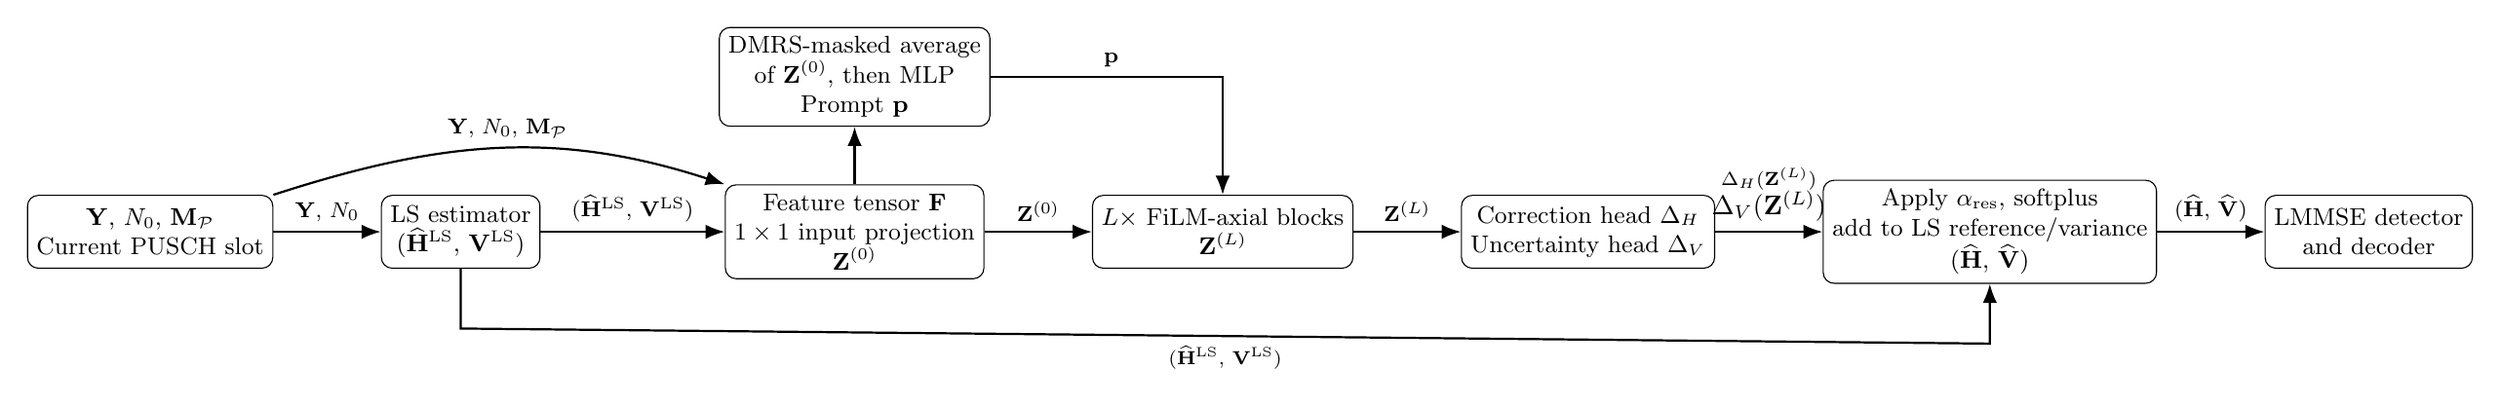
\begin{tikzpicture}[
				node distance=0.9cm and 1.4cm,
				block/.style={draw, rounded corners, minimum height=0.95cm, minimum width=2.0cm, align=center, font=\small},
				smallblock/.style={draw, rounded corners, minimum height=0.85cm, minimum width=1.8cm, align=center, font=\small},	arr/.style={-{Latex[length=2.5mm]}, thick}	]
				\node[block] (slot) {$\mathbf{Y},\,N_0,\,\mathbf{M}_{\mathcal{P}}$\\Current PUSCH slot};
				\node[block, right=of slot] (ls) {LS estimator\\$(\widehat{\mathbf{H}}^{\mathrm{LS}},\,\mathbf{V}^{\mathrm{LS}})$};
				\node[block, right=2.4cm of ls] (feat) {Feature tensor $\mathbf{F}$\\$1\times1$ input projection\\$\mathbf{Z}^{(0)}$};
				\node[smallblock, above=0.75cm of feat] (prompt) {DMRS-masked average\\of $\mathbf{Z}^{(0)}$, then MLP\\Prompt $\mathbf{p}$};
				\node[block, right=of feat] (blocks) {$L\times$ FiLM-axial blocks\\$\mathbf{Z}^{(L)}$};
				\node[block, right=of blocks] (heads) {Correction head $\Delta_H$\\Uncertainty head $\Delta_V$};
				\node[block, right=of heads] (merge) {Apply $\alpha_{\mathrm{res}}$, softplus\\add to LS reference/variance\\$(\widehat{\mathbf{H}},\,\widehat{\mathbf{V}})$};
				\node[block, right=of merge] (det) {LMMSE detector\\and decoder};
				
				\path (ls.south) ++(0,-0.78cm) coordinate (ls_aux);
				\path (merge.south) ++(0,-0.78cm) coordinate (merge_aux);
				
				\draw[arr] (slot) -- node[midway, above] {\footnotesize $\mathbf{Y},\,N_0$} (ls);
				\draw[arr] (ls) -- node[midway, above] {\footnotesize $(\widehat{\mathbf{H}}^{\mathrm{LS}},\,\mathbf{V}^{\mathrm{LS}})$} (feat);
				\draw[arr] (slot.north east) to[out=18,in=162] node[pos=0.52, above] {\footnotesize $\mathbf{Y},\,N_0,\,\mathbf{M}_{\mathcal{P}}$} (feat.north west);
				\draw[arr] (feat) -- node[midway, above] {\footnotesize $\mathbf{Z}^{(0)}$} (blocks);
				\draw[arr] (blocks) -- node[midway, above] {\footnotesize $\mathbf{Z}^{(L)}$} (heads);
				\draw[arr] (heads) -- node[midway, above, align=center] {\scriptsize $\Delta_H(\mathbf{Z}^{(L)})$\\[-1pt]$\Delta_V(\mathbf{Z}^{(L)})$} (merge);
				\draw[arr] (merge) -- node[midway, above] {\footnotesize $(\widehat{\mathbf{H}},\,\widehat{\mathbf{V}})$} (det);
				\draw[arr] (ls.south) -- (ls_aux) -- node[midway, below] {\scriptsize $(\widehat{\mathbf{H}}^{\mathrm{LS}},\,\mathbf{V}^{\mathrm{LS}})$} (merge_aux) -- (merge.south);
				\draw[arr] (feat.north) -- (prompt.south);
				\draw[arr] (prompt.east) -| node[pos=0.26, above] {\footnotesize $\mathbf{p}$} (blocks.north);
			\end{tikzpicture}%
		}
		\caption{UPAIR receiver flow. The LS output and current slot observations are mapped to $\mathbf{F}$, projected to $\mathbf{Z}^{(0)}$, summarized over DMRS to form the prompt $\mathbf{p}$, refined by $L$ FiLM-axial blocks, and output as $(\widehat{\mathbf{H}},\widehat{\mathbf{V}})$ for the standard LMMSE detector. Figs.~\ref{fig:prompted_block} and~\ref{fig:film_detail} detail one axial block and the FiLM step.}
		\label{fig:pipeline}
	\end{figure*}
	
	\section{UPAIR Channel-Estimation front-end}
	\label{sec:upair_model}
	
	%	Figure~\ref{fig:pipeline} summarizes the UPAIR{} pipeline.
	%	The estimator takes the current slot observations $(\mathbf{Y}, N_0, \mathbf{M}_{\mathcal{P}})$ and the LS reference $(\widehat{\mathbf{H}}^{\mathrm{LS}}, \mathbf{V}^{\mathrm{LS}})$ as inputs and produces a refined channel estimate $\widehat{\mathbf{H}}$ and an uncertainty map $\widehat{\mathbf{V}}$.
	%	It proceeds in four steps: (i)~feature construction, (ii)~slot prompt extraction, (iii)~FiLM-conditioned axial refinement, and (iv)~output head projections.
	%	Each step is detailed below.
	%Figure~\ref{fig:pipeline} summarizes the UPAIR{} pipeline.
	%The estimator takes the current slot observations $(\mathbf{Y}, N_0, \mathbf{M}_{\mathcal{P}})$ and the LS reference $(\widehat{\mathbf{H}}^{\mathrm{LS}}, \mathbf{V}^{\mathrm{LS}})$ as inputs and produces a refined channel estimate $\widehat{\mathbf{H}}$ and an uncertainty map $\widehat{\mathbf{V}}$.
	%It proceeds in four steps: (i)~feature construction, (ii)~slot prompt extraction, (iii)~FiLM-conditioned axial refinement, and (iv)~output head projections.
	%Step (iii) consists of $L$ stacked \emph{axial blocks}, each transforming a running state $\mathbf{X}_i\in\mathbb{R}^{T\times F\times d}$ through four sub-stages, namely two axial self-attentions, a depthwise-pointwise convolution, and a pointwise MLP, combined via residual connections; the slot prompt $\mathbf{p}$ enters each sub-stage through FiLM conditioning.
	Figure~\ref{fig:pipeline} summarizes the UPAIR{} pipeline.
	The estimator takes the current slot observations $(\mathbf{Y}, N_0, \mathbf{M}_{\mathcal{P}})$ and the LS reference $(\widehat{\mathbf{H}}^{\mathrm{LS}}, \mathbf{V}^{\mathrm{LS}})$ as inputs and produces a refined channel estimate $\widehat{\mathbf{H}}$ and an uncertainty map $\widehat{\mathbf{V}}$.
	It proceeds in four steps: (i)~feature construction, (ii)~slot prompt extraction, (iii)~FiLM-conditioned axial refinement, and (iv)~output head projections.
	Step (iii) consists of $L$ stacked \emph{axial blocks}; within each block, a state tensor $\mathbf{X}\in\mathbb{R}^{T\times F\times d}$ is updated across four sub-stages, namely two axial self-attentions, a depthwise-pointwise convolution, and a pointwise MLP, each with a residual connection and FiLM conditioning by the slot prompt $\mathbf{p}$.
	\vspace{-.1cm}
	\subsection{Feature construction}
	\label{subsec:features}
	The estimator first converts the available slot information into a single
	real-valued feature tensor. For
	$\mathbf{A}\in\mathbb{C}^{T\times F\times N_r}$, define the
	real--imaginary stacking operator
	$\mathcal{R}(\mathbf{A})
	\triangleq
	\operatorname{concat}_{\rm feat}(\Re\{\mathbf{A}\},\Im\{\mathbf{A}\})
	\in\mathbb{R}^{T\times F\times 2N_r}$,
	which stacks the real and imaginary parts of the $N_r$ receive-antenna
	slices along the feature axis. Then,
	\begin{equation}
		\small
		\label{eq:feature_tensor}
		\begin{aligned}
			\mathbf{F}
			&=
			\operatorname{concat}_{\rm feat}\!\left(
			\mathcal{R}(\widehat{\mathbf{H}}^{\mathrm{LS}}),
			\mathcal{R}(\mathbf{Y}),
			\overline{\mathbf{V}}^{\mathrm{LS}},
			\mathbf{N}_0,
			\mathbf{M}_{\mathcal{P}}^{\rm map}
			\right) \\
			&\in
			\mathbb{R}^{T\times F\times(4N_r+3)} .
		\end{aligned}
	\end{equation}
	%	Here, $\operatorname{concat}_{\rm feat}(\cdot)$ denotes concatenation along
	%	the third, feature dimension, $\mathbf{N}_0=N_0\mathbf{1}_{T\times F\times 1}$,
	%	and $\mathbf{M}_{\mathcal{P}}^{\rm map}$ is the $T\times F$ pilot mask viewed
	%	as a $T\times F\times1$ map. Thus the feature dimension is
	%	$4N_r+3$, e.g., $11$ for $N_r=2$.
	Here, $\operatorname{concat}_{\rm feat}(\cdot)$ denotes concatenation along the third (feature) dimension, $\overline{\mathbf{V}}^{\mathrm{LS}}\in\mathbb{R}_{+}^{T\times F\times 1}$ is $\mathbf{V}^{\mathrm{LS}}$ averaged over the $N_r$ receive-antenna axis, $\mathbf{N}_0=N_0\mathbf{1}_{T\times F\times 1}$, and $\mathbf{M}_{\mathcal{P}}^{\rm map}\in\{0,1\}^{T\times F\times 1}$ is the pilot mask viewed as a $T\times F\times 1$ map. The feature dimension is therefore $4N_r+3$, e.g., $11$ for $N_r=2$.
	
	A $1\times1$ convolution then projects each per-$(t,f)$ feature vector to dimension $d$. That is,
	\begin{equation}
		\label{eq:stem}
		\big[\mathbf{Z}^{(0)}\big]_{t,f,:}
		=
		\mathbf{W}_{\rm con}
		\big[\mathbf{F}\big]_{t,f,:}
		+
		\mathbf{b}_{\rm con},
		\qquad
		\mathbf{Z}^{(0)}\in\mathbb{R}^{T\times F\times d},
	\end{equation}
	where
	$\mathbf{W}_{\rm con}\in\mathbb{R}^{d\times(4N_r+3)}$
	and
	$\mathbf{b}_{\rm con}\in\mathbb{R}^{d}$.
	The feature tensor $\mathbf{Z}^{(0)}$ is the shared starting point for both the slot-prompt extraction and the subsequent axial refinement.
	\vspace{-.2cm}
	\subsection{Slot-prompt extraction}
	\label{subsec:prompt}
	
	The slot prompt $\mathbf{p}\in\mathbb{R}^{d}$ is a compact vector that summarizes the channel conditions of the current slot using only the reliable DMRS positions.
	It is obtained by averaging the projected features over all pilot locations $\mathcal{P}$ and passing the result through a two-layer MLP $g_\psi$. Particularly,
	\begin{equation}
		\label{eq:prompt_pool}
		\mathbf{p}
		=
		g_{\psi}\!\left(
		\frac{1}{|\mathcal{P}|}
		\sum_{(t,f)\in\mathcal{P}} \mathbf{Z}^{(0)}_{t,f,:}
		\right).
	\end{equation}
	The prompt uses only DMRS positions, avoiding noisy data REs, and is computed once per slot.
	%It encodes the current-slot channel quality into a single vector that steers all downstream blocks via FiLM.
	%	\vspace{-.4cm}
	\vspace{-.2cm}
	\subsection{FiLM-conditioned axial refinement}
	\label{subsec:axial_refinement}
	
	\subsubsection{FiLM conditioning}
	At the beginning of each sub-stage inside every axial block, the current block state $\mathbf{X}_i\in\mathbb{R}^{T\times F\times d}$ is normalized and modulated by the slot prompt.
	First, the prompt is projected to a gain vector $\boldsymbol{\gamma}(\mathbf{p})\in\mathbb{R}^{d}$ and a bias vector as $\boldsymbol{\beta}(\mathbf{p})\in\mathbb{R}^{d}$
	\begin{equation}
		\label{eq:film_params}
		\bigl[\boldsymbol{\gamma}(\mathbf{p}),\;\boldsymbol{\beta}(\mathbf{p})\bigr]
		=
		\operatorname{split}\!\left(\mathbf{W}_{p}\mathbf{p}+\mathbf{b}_{p}\right),
	\end{equation}
	where $\mathbf{W}_{p}\in\mathbb{R}^{2d\times d}$ and $\mathbf{b}_{p}\in\mathbb{R}^{2d}$ are learned parameters, and $\operatorname{split}(\cdot)$ partitions the $2d$-dimensional output into two $d$-dimensional halves.
	The FiLM-conditioned tensor is then formed by applying these vectors uniformly to every resource element $(t,f)$ according to
	\begin{equation}
		\label{eq:film}
		[\widetilde{\mathbf{X}}_i]_{t,f,:}
		=
		\operatorname{LN}\!\bigl([\mathbf{X}_i]_{t,f,:}\bigr)
		\odot
		\bigl(\mathbf{1}+\boldsymbol{\gamma}(\mathbf{p})\bigr)
		+
		\boldsymbol{\beta}(\mathbf{p}),
	\end{equation}
	where $\operatorname{LN}(\cdot)$ denotes layer normalization applied independently at each $(t,f)$ position, normalizing the $d$-dimensional feature vector $[\mathbf{X}_i]_{t,f,:}$ to zero mean and unit variance over the feature axis, and $\odot$ is element-wise multiplication. 	Because $\boldsymbol{\gamma}$ and $\boldsymbol{\beta}$ are computed from $\mathbf{p}$ and broadcast over all $(t,f)$, the same slot-level modulation is applied uniformly across the entire resource grid. 
The resulting tensor $\widetilde{\mathbf{X}}_i$ is the input to the $i$th sub-stage of the block. Figure~\ref{fig:film_detail} illustrates this operation, applied inside the ``$L\times$ FiLM-axial blocks'' of Fig.~\ref{fig:pipeline}.

%Figure~\ref{fig:film_detail} illustrates this operation.

%Figure~\ref{fig:film_detail} illustrates this operation, which is invoked inside the ``$L\times$ FiLM-axial blocks'' box of Fig.~\ref{fig:pipeline} at the start of every sub-stage.
	%
	%
	
	\subsubsection{Axial block structure}
	Each FiLM-conditioned axial block transforms the input tensor $\mathbf{X}_0 = \mathbf{Z}^{(\ell)}\in\mathbb{R}^{T\times F\times d}$ through four sequential sub-stages, each with a residual skip connection, yielding the block output $\mathbf{X}_4 = \mathbf{Z}^{(\ell+1)}$.
	The term \emph{axial} refers to the fact that self-attention is applied one-dimensionally along a single axis of the resource grid at a time, either across the $F$ subcarriers within a fixed OFDM symbol, or across the $T$ OFDM symbols at a fixed subcarrier (rather than jointly over the full two-dimensional grid). This factorization not only matches the separable time-frequency structure of OFDM, but also reduces the computational complexity from $O((TF)^2)$ to $O(T F^2 + F T^2)$.
	The four sub-stages are as follows (see also Fig.~\ref{fig:prompted_block}).
	
	\textbf{Sub-stage 1 --- Frequency self-attention.}
	The FiLM-conditioned slice $[\widetilde{\mathbf{X}}_0]_{t,:,:}\in\mathbb{R}^{F\times d}$ at each OFDM symbol $t$ is processed by a multi-head self-attention (MHA) module applied independently across the $F$ subcarriers.
	Let $\mathbf{Q},\mathbf{K},\mathbf{V}\in\mathbb{R}^{F\times d}$ denote the query, key, and value projections of this slice.
	The scaled dot-product attention output for symbol $t$ is
	\vspace{-.3cm}
	\begin{equation}
		\label{eq:freq_attn}
		\mathcal{A}_{f}^{t}
		=
		\operatorname{softmax}\!\!\left(\frac{\mathbf{Q}\mathbf{K}^{\top}}{\sqrt{d/H}}\right)\mathbf{V}
		\;\in\mathbb{R}^{F\times d},
	\end{equation}
	where $H$ is the number of attention heads and $d/H$ is the per-head dimension.
	After processing all $T$ symbols independently, the outputs are stacked back to the full grid and added to $\mathbf{X}_0$ through a residual connection $	\mathbf{X}_1 = \mathbf{X}_0 + \operatorname{Drop}_\rho(\mathcal{A}_{f}(\widetilde{\mathbf{X}}_0))$,
	%	\begin{equation}
		%		\mathbf{X}_1 = \mathbf{X}_0 + \operatorname{Drop}_\rho(\mathcal{A}_{f}(\widetilde{\mathbf{X}}_0)),
		%	\end{equation}
	where $\operatorname{Drop}_\rho(\cdot)$ denotes dropout with rate $\rho$ (active only during training, identity at inference), and $\mathcal{A}_{f}(\widetilde{\mathbf{X}}_0)$ stacks the per-symbol outputs $\mathcal{A}_{f}^{t}$ over all $t$.
	This sub-stage allows every subcarrier to attend to all other subcarriers within the same symbol, capturing frequency-domain channel correlations.
	
	\textbf{Sub-stage 2 --- Time self-attention.}
	The same MHA operation is now applied along the time axis.
	The FiLM-conditioned slice $[\widetilde{\mathbf{X}}_1]_{:,f,:}\in\mathbb{R}^{T\times d}$ at each subcarrier $f$ is processed independently, yielding the per-subcarrier time-attention output $\mathcal{A}_{t}^{f}\in\mathbb{R}^{T\times d}$.
	After stacking over all $f$, we have 		$\mathbf{X}_2 = \mathbf{X}_1 + \operatorname{Drop}_\rho(\mathcal{A}_{t}(\widetilde{\mathbf{X}}_1))$.
	%	\begin{equation}
		%		\mathbf{X}_2 = \mathbf{X}_1 + \operatorname{Drop}_\rho(\mathcal{A}_{t}(\widetilde{\mathbf{X}}_1)).
		%	\end{equation}
	This sub-stage lets every OFDM symbol attend to all other symbols at the same subcarrier, capturing temporal channel variations.
	
	\textbf{Sub-stage 3 --- Depthwise-pointwise convolution.}
	To capture short-range local structure in the time-frequency grid, this sub-stage applies a depth-separable convolution to $\widetilde{\mathbf{X}}_2$.
	A depthwise $3\times3$ convolution (DWConv) processes each of the $d$ feature maps independently, applying one distinct $3\times3$ spatial kernel $k_c$ to each feature map.
	
	A pointwise $1\times1$ convolution (PWConv) then mixes the $d$ features independently at each resource element. Let $\mathbf{U}_{t,f,:}\in\mathbb{R}^{d}$ denote the local feature vector at $(t,f)$. The operation is
	\begin{equation}
		\label{eq:pwconv}
		[\operatorname{PWConv}(\mathbf{U})]_{t,f,:}
		=
		\mathbf{W}\mathbf{U}_{t,f,:}+\mathbf{b},
	\end{equation}
	where $\mathbf{W}\in\mathbb{R}^{d\times d}$ and $\mathbf{b}\in\mathbb{R}^d$ are shared across all $(t,f)$.
	The branch output is $\mathcal{C}(\widetilde{\mathbf{X}}_2)=\operatorname{Drop}_\rho(\operatorname{GELU}(\operatorname{PWConv}(\operatorname{DWConv}(\widetilde{\mathbf{X}}_2))))$, and the residual update is $\mathbf{X}_3 = \mathbf{X}_2 + \mathcal{C}(\widetilde{\mathbf{X}}_2)$.
	Together, DWConv and PWConv form a depthwise-separable convolution: DWConv captures local structure, and PWConv mixes features per position.
	
	
	\textbf{Sub-stage 4 --- Pointwise MLP.}
	A small MLP is applied independently at every $(t,f)$ position to mix features. It expands the $d$-dimensional feature vector to dimension $rd$ via a fully connected layer FC$_1$ (expansion ratio $r$), applies GELU \cite{gelu} and dropout, then projects back to $d$ via FC$_2$ followed by another dropout. This can be written compactly as
	%\begin{equation}
	%	\mathcal{M}(\widetilde{\mathbf{X}}_3)
	%	=
	%	\operatorname{Drop}_\rho\!\bigl(\operatorname{FC}_2(\operatorname{Drop}_\rho(\operatorname{GELU}(\operatorname{FC}_1(\widetilde{\mathbf{X}}_3))))\bigr),
	%\end{equation}
	\begin{equation}
		\small
		\label{eq:pointwise_mlp}
		\begin{aligned}
			\big[\mathcal{M}(\widetilde{\mathbf{X}}_3)\big]_{t,f,:}
			&= \\
			&\hspace{-5.5em}\operatorname{Drop}_{\rho}\!\left(
			\mathbf{W}_2
			\operatorname{Drop}_{\rho}\!\left(
			\operatorname{GELU}\!\left(
			\mathbf{W}_1[\widetilde{\mathbf{X}}_3]_{t,f,:}
			+\mathbf{b}_1
			\right)
			\right)
			+\mathbf{b}_2
			\right),
		\end{aligned}
	\end{equation}
	where FC$_1$ and FC$_2$ use weight matrices $\mathbf{W}_1\in\mathbb{R}^{rd \times d}$ and $\mathbf{W}_2\in\mathbb{R}^{d \times rd}$, and bias vectors $\mathbf{b}_1\in\mathbb{R}^{rd}$ and $\mathbf{b}_2\in\mathbb{R}^{d}$ respectively, shared across all $(t,f)$. The residual update gives the block output $\mathbf{X}_4
	=
	\mathbf{Z}^{(\ell+1)}
	=
	\mathbf{X}_3 + \mathcal{M}(\widetilde{\mathbf{X}}_3).$
	%	It is worth stressing that the blocks labeled ``Dropout'' are present only during training and have no effect at inference.
	Stacking $L$ such blocks yields the final representation
	$\mathbf{Z}^{(L)} = \mathcal{B}_{L-1}\!\left(\cdots\mathcal{B}_0\!\left(\mathbf{Z}^{(0)};\mathbf{p}\right)\cdots;\mathbf{p}\right)$,
	where $\mathcal{B}_\ell(\cdot\,;\mathbf{p})$ denotes the $\ell$th block conditioned on the slot prompt $\mathbf{p}$.
	
	
	\begin{figure}[t]
		\centering
		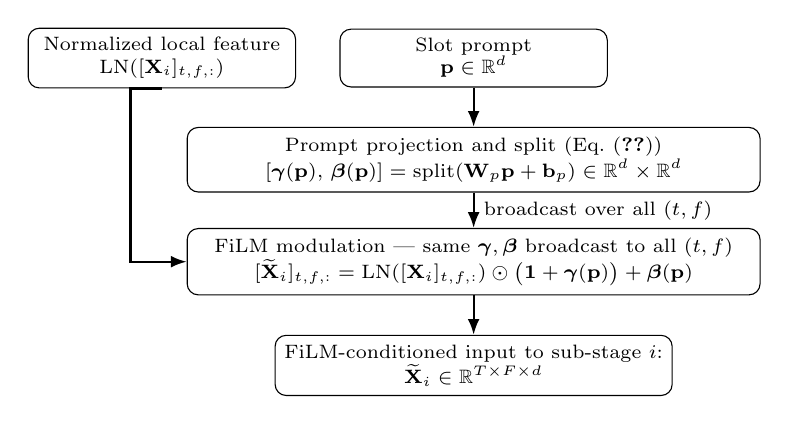
\begin{tikzpicture}[
			node distance=0.45cm and 0.55cm,
			box/.style={draw, rounded corners, minimum width=0.60\columnwidth, minimum height=0.82cm, align=center, font=\scriptsize},
			small/.style={draw, rounded corners, minimum width=0.28\columnwidth, minimum height=0.72cm, align=center, font=\scriptsize},
			arr/.style={-{Latex[length=2.0mm]}, thick}
			]
			\node[small] (zin) {Normalized local feature\\$\operatorname{LN}([\mathbf{X}_i]_{t,f,:})$};
			\node[small, right=of zin] (p) {Slot prompt\\$\mathbf{p}\in\mathbb{R}^d$};
			
			\node[box, below=0.50cm of p] (proj) {Prompt projection and split (Eq.~\eqref{eq:film_params})\\
				$\left[\boldsymbol{\gamma}(\mathbf{p}),\,\boldsymbol{\beta}(\mathbf{p})\right]
				=
				\operatorname{split}\!\left(\mathbf{W}_{p}\mathbf{p}+\mathbf{b}_{p}\right)\in\mathbb{R}^d\times\mathbb{R}^d$};
			
			\node[box, below=0.45cm of proj] (film) {FiLM modulation --- same $\boldsymbol{\gamma},\boldsymbol{\beta}$ broadcast to all $(t,f)$\\
				$[\widetilde{\mathbf{X}}_i]_{t,f,:}
				=
				\operatorname{LN}([\mathbf{X}_i]_{t,f,:})\odot\big(\mathbf{1}+\boldsymbol{\gamma}(\mathbf{p})\big)
				+\boldsymbol{\beta}(\mathbf{p})$};
			
			\node[small, below=0.5cm of film] (zout) {FiLM-conditioned input to sub-stage $i$:\\$\widetilde{\mathbf{X}}_i\in\mathbb{R}^{T\times F\times d}$};
			
			\draw[arr] (p.south) -- (proj.north);
			\draw[arr] (proj) -- node[midway, right, font=\scriptsize] {broadcast over all $(t,f)$} (film);
			\draw[arr] (zin.south) -- ++(-0.4cm,0) |- (film.west);
			\draw[arr] (film) -- (zout);
		\end{tikzpicture}
		\caption{FiLM conditioning applied at the $i$th sub-stage of each axial block.}
		\label{fig:film_detail}
		%The slot prompt $\mathbf{p}$ is projected to a gain $\boldsymbol{\gamma}$ and bias $\boldsymbol{\beta}$, which are broadcast uniformly across all $T\times F$ resource elements to produce the conditioned tensor $\widetilde{\mathbf{X}}_i$ (Eq.~\eqref{eq:film}).
	\end{figure}
	
	\begin{figure}[t]
		\centering
		\resizebox{1\columnwidth}{!}{%
			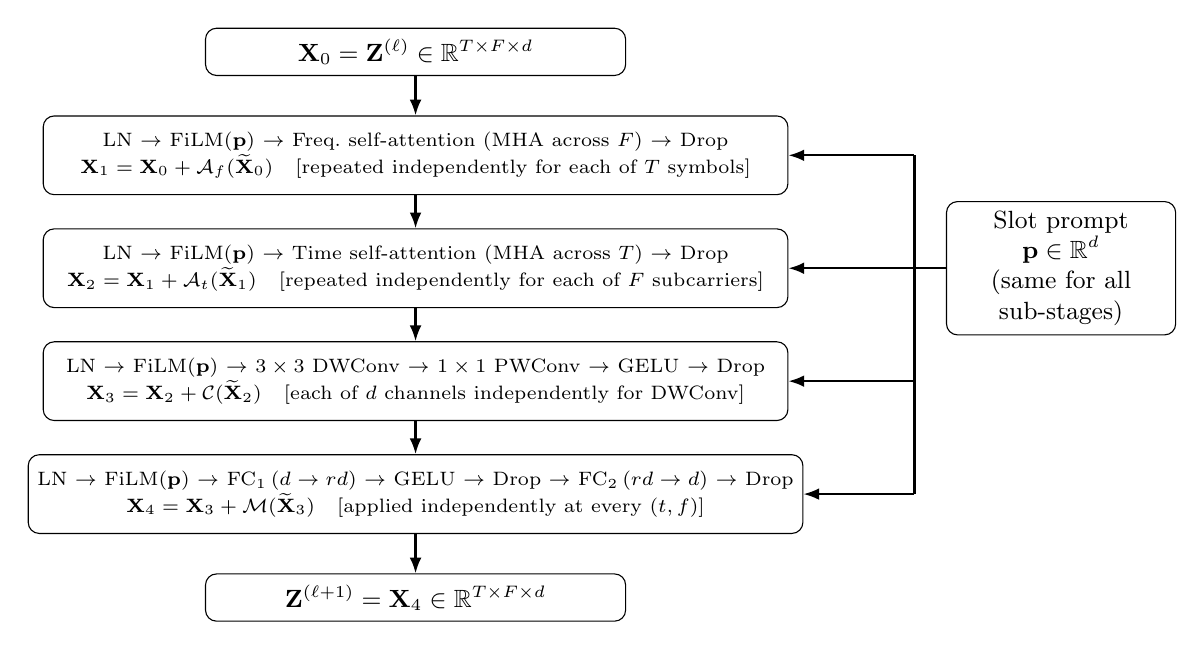
\begin{tikzpicture}[
				node distance=0.44cm,
				state/.style={draw, rounded corners, minimum width=0.44\columnwidth, minimum height=0.60cm, align=center, font=\small},
				stage/.style={draw, rounded corners, minimum width=0.78\columnwidth, minimum height=1.00cm, align=center, font=\scriptsize},
				side/.style={draw, rounded corners, minimum width=0.24\columnwidth, minimum height=0.78cm, align=center, font=\small},
				arr/.style={-{Latex[length=2.0mm]}, thick}
				]
				\node[state] (x0) at (0.8cm,0) {$\mathbf{X}_0=\mathbf{Z}^{(\ell)}\in\mathbb{R}^{T\times F\times d}$};
				
				\node[stage, below=0.50cm of x0] (f1) {LN $\to$ FiLM($\mathbf{p}$) $\to$ Freq.\ self-attention (MHA across $F$) $\to$ Drop\\
					$\mathbf{X}_1=\mathbf{X}_0+\mathcal{A}_{f}(\widetilde{\mathbf{X}}_0)$\quad[repeated independently for each of $T$ symbols]};
				
				\node[stage, below=0.42cm of f1] (f2) {LN $\to$ FiLM($\mathbf{p}$) $\to$ Time self-attention (MHA across $T$) $\to$ Drop\\
					$\mathbf{X}_2=\mathbf{X}_1+\mathcal{A}_{t}(\widetilde{\mathbf{X}}_1)$\quad[repeated independently for each of $F$ subcarriers]};
				
				\node[stage, below=0.42cm of f2] (f3) {LN $\to$ FiLM($\mathbf{p}$) $\to$ $3\times3$ DWConv $\to$ $1\times1$ PWConv $\to$ GELU $\to$ Drop\\
					$\mathbf{X}_3=\mathbf{X}_2+\mathcal{C}(\widetilde{\mathbf{X}}_2)$\quad[each of $d$ channels independently for DWConv]};
				
				\node[stage, below=0.42cm of f3] (f4) {LN $\to$ FiLM($\mathbf{p}$) $\to$ FC$_1\,(d\to rd)$ $\to$ GELU $\to$ Drop $\to$ FC$_2\,(rd\to d)$ $\to$ Drop\\
					$\mathbf{X}_4=\mathbf{X}_3+\mathcal{M}(\widetilde{\mathbf{X}}_3)$\quad[applied independently at every $(t,f)$]};
				
				\node[state, below=0.50cm of f4] (x4) {$\mathbf{Z}^{(\ell+1)}=\mathbf{X}_4\in\mathbb{R}^{T\times F\times d}$};
				
				\node[side, right=2.0cm of f2] (p) {Slot prompt\\$\mathbf{p}\in\mathbb{R}^d$\\(same for all\\sub-stages)};
				
				\draw[arr] (x0) -- (f1);
				\draw[arr] (f1) -- (f2);
				\draw[arr] (f2) -- (f3);
				\draw[arr] (f3) -- (f4);
				\draw[arr] (f4) -- (x4);
				
				\coordinate (spine) at ($(f2.east) + (1.60cm, 0)$);
				\draw[thick] (spine |- f1) -- (spine |- f4);
				\draw[thick] (p.west) -- (spine |- p.west);
				\draw[arr] (spine |- f1) -- (f1.east);
				\draw[arr] (spine |- f2) -- (f2.east);
				\draw[arr] (spine |- f3) -- (f3.east);
				\draw[arr] (spine |- f4) -- (f4.east);
				
			\end{tikzpicture}%
		}
		\caption{One FiLM-conditioned axial block $\mathcal{B}_\ell$. }
		\label{fig:prompted_block}
		%The four sub-stages---frequency attention, time attention, depthwise-pointwise convolution, and pointwise MLP---each apply LN $\to$ FiLM($\mathbf{p}$) before their main operation and add the result back to the running tensor via a residual skip connection. Dropout layers are active only during training. The same slot prompt $\mathbf{p}$ conditions all four sub-stages.
	\end{figure}
	\vspace{-.2cm}
	\subsection{Correction and uncertainty output heads}
	\label{subsec:output_heads}
	\label{subsec:training}	
	%After the last axial block, the final tensor $\mathbf{Z}^{(L)}\in\mathbb{R}^{T\times F\times d}$ is projected by two parallel $1\times1$ convolutional heads.
	%Both heads are pointwise maps (i.e., they operate independently at every $(t,f)$, sharing the same weights across the grid).
	The final tensor $\mathbf{Z}^{(L)}\in\mathbb{R}^{T\times F\times d}$ is projected by two parallel $1\times1$ convolutional heads:
	
	\textbf{Correction head} $\Delta_H$: A $1\times1$ convolution projects $\mathbf{Z}^{(L)}$ from feature dimension $d$ to $2N_r$ real-valued outputs, grouped into real and imaginary parts to form a complex correction $\Delta_H(\mathbf{Z}^{(L)})\in\mathbb{C}^{T\times F\times N_r}$.
	The refined channel estimate is
	\begin{equation}
		\label{eq:residual_head}
		\widehat{\mathbf{H}}
		=
		\widehat{\mathbf{H}}^{\mathrm{LS}}
		+
		\alpha_{\mathrm{res}}\,\Delta_H\!\left(\mathbf{Z}^{(L)}\right),
	\end{equation}
	where $\alpha_{\mathrm{res}}$ is a fixed chosen correction scale factor.
	
	\textbf{Uncertainty head} $\Delta_V$: A separate $1\times1$ convolution maps $d$ to $N_r$ real values.
	The refined uncertainty map is
	\begin{equation}
		\label{eq:variance_head}
		\widehat{\mathbf{V}}
		=
		\mathbf{V}^{\mathrm{LS}}
		+
		\operatorname{softplus}\!\left(\Delta_V\!\left(\mathbf{Z}^{(L)}\right)\right),
	\end{equation}
	where $\operatorname{softplus}(x)=\log(1+e^x)\geq 0$. The uncertainty head selectively increases the estimated variance in unreliable regions, which directly affects the downstream LMMSE detector.
	The pair $(\widehat{\mathbf{H}},\widehat{\mathbf{V}})$ is passed to the standard downstream LMMSE detector without any further modification.
	\vspace{-.1cm}
	\subsection{Training objective}
	During training, the estimator is trained end-to-end on freshly generated PUSCH slots.
	For each slot, the ground-truth channel tensor $\mathbf{H}$ is available from the channel simulator.
	The loss combines a variance-weighted squared error (with a $\log\widehat{\mathbf{V}}$ term that prevents $\widehat{\mathbf{V}}$ from collapsing to zero) and a normalized MSE (NMSE) regularizer as
	\begin{equation}
		\label{eq:training_loss}
		\small
		\mathcal{L}
		=
		\underbrace{
			\operatorname{mean}\!\!\left(
			\frac{\left|\mathbf{H}-\widehat{\mathbf{H}}\right|^2}{\widehat{\mathbf{V}}+\varepsilon}
			+
			\log\!\left(\widehat{\mathbf{V}}+\varepsilon\right)
			\right)
		}_{\text{variance-weighted SE}}
		+
		\lambda\,
		\underbrace{
			\frac{
				\operatorname{mean}\!\left(\left|\mathbf{H}-\widehat{\mathbf{H}}\right|^2\right)
			}{
				\operatorname{mean}\!\left(\left|\mathbf{H}\right|^2\right)+\varepsilon
			}
		}_{\text{NMSE regularizer}},
	\end{equation}
%	The loss combines a heteroscedastic Gaussian negative log-likelihood (NLL) term with an normalized MSE (NMSE) regularizer as
%	\begin{equation}
%		\label{eq:training_loss}
%		\small
%		\mathcal{L}
%		=
%		\underbrace{
%			\operatorname{mean}\!\!\left(
%			\frac{\left|\mathbf{H}-\widehat{\mathbf{H}}\right|^2}{\widehat{\mathbf{V}}+\varepsilon}
%			+
%			\log\!\left(\widehat{\mathbf{V}}+\varepsilon\right)
%			\right)
%		}_{\text{heteroscedastic NLL}}
%		+
%		\lambda\,
%		\underbrace{
%			\frac{
%				\operatorname{mean}\!\left(\left|\mathbf{H}-\widehat{\mathbf{H}}\right|^2\right)
%			}{
%				\operatorname{mean}\!\left(\left|\mathbf{H}\right|^2\right)+\varepsilon
%			}
%		}_{\text{NMSE regularizer}},
%	\end{equation}
	where $\varepsilon>0$ is a numerical-stability constant and $\lambda$ weights the NMSE term.
	The NLL term jointly trains the correction head and the uncertainty head: it encourages $\widehat{\mathbf{H}}$ to approach $\mathbf{H}$ while $\widehat{\mathbf{V}}$ reflects the actual error magnitude.
	%The NMSE regularizer provides a direct gradient signal on the channel error.
	%The squared magnitude, division, and logarithm in the NLL are applied elementwise over the channel coefficients before the final mean.
	Training uses an adaptive optimizer with weight decay, gradient clipping, and checkpointing of the best validation model.
	
	
	\paragraph*{Remark.}
	%	The refined pair $(\widehat{\mathbf{H}},\widehat{\mathbf{V}})$ is consumed directly by the unchanged downstream LMMSE detector. In the single-layer setting considered in this paper, for each resource element $(t,f)$, the detector uses $\widehat{H}_{t,f,r}$ as the channel estimate on receive antenna $r$ and uses $\widehat{V}_{t,f,r}$ as the corresponding CSI-uncertainty variance. Hence, $\widehat{\mathbf{V}}$ enters the detector as an additional diagonal term to the noise variance $N_0$, so that antennas or resource elements with larger estimated uncertainty are trusted less. 
	The pair $(\widehat{\mathbf{H}},\widehat{\mathbf{V}})$ feeds directly into the unchanged LMMSE detector: $\widehat{V}_{t,f,r}$ acts as a diagonal addition to $N_0$, so resource elements with larger estimated uncertainty are weighted less. The resulting post-equalized symbol can be written as
	\begin{equation}
		\label{eq:lmmse_consumption_symbol}
		\widehat{x}_{t,f}
		=
		\frac{\displaystyle\sum_{r=1}^{N_r}
			\frac{\widehat{H}^{*}_{t,f,r}}{N_0+\widehat{V}_{t,f,r}}\,y_{t,f,r}}
		{\displaystyle\sum_{r=1}^{N_r}
			\frac{\left|\widehat{H}_{t,f,r}\right|^2}{N_0+\widehat{V}_{t,f,r}}},
	\end{equation}
	with corresponding effective post-equalization noise variance
	\begin{equation}
		\label{eq:lmmse_consumption_var}
		\sigma^2_{t,f}
		=
		\left(
		\sum_{r=1}^{N_r}
		\frac{\left|\widehat{H}_{t,f,r}\right|^2}{N_0+\widehat{V}_{t,f,r}}
		\right)^{-1}.
	\end{equation}
	The pair $(\widehat{x}_{t,f},\sigma^2_{t,f})$ is then passed to the standard soft demapper to produce the bit LLRs. 
	
	\vspace{-.2cm}
	\section{Baselines}
	\label{sec:baselines}
	
	%\subsection{}
	%\label{subsec:classical}
	The practical baselines we used are the standard LS, LS + 2D LMMSE, and an LS baseline augmented with decision-directed common-phase-error correction~\cite{Abhayawardhana2002,Liao2006}. The LS + 2D LMMSE receiver replaces the default LS interpolation by a separable LMMSE interpolator built from empirical covariance matrices $\mathbf{R}_t$, $\mathbf{R}_f$, and $\mathbf{R}_s$, estimated offline from generated channel realizations, with interpolation order frequency--time--space.
	
	For the DD-CPE{} baseline, the iteration is initialized by $\widehat{\mathbf{H}}^{(0)}=\widehat{\mathbf{H}}^{\mathrm{LS}}$. At iteration $i$, the equalized symbol is
	\begin{equation}
		\label{eq:ddcpe_equalizer}
		z^{(i)}_{t,f}
		=
		\frac{
			\sum_{r=1}^{N_r}\big(\widehat{h}^{(i)}_{t,f,r}\big)^{*} y_{t,f,r}
		}{
			\sum_{r=1}^{N_r}\left|\widehat{h}^{(i)}_{t,f,r}\right|^2 + N_0
		}.
	\end{equation}
	Using the hard decision $\widehat{s}^{(i)}_{t,f}$, one residual common phase per OFDM symbol is estimated as
	\begin{equation}
		\label{eq:ddcpe_metric}
		\widehat{\theta}^{(i)}_{t}
		=
		\angle\!\left(
		\sum_{f\in\mathcal{D}_t}
		\left(
		\sum_{r=1}^{N_r}\left|\widehat{h}^{(i)}_{t,f,r}\right|^2 
		\right)^{\eta}
		z^{(i)}_{t,f}\,\big(\widehat{s}^{(i)}_{t,f}\big)^{*}
		\right),
		%+ \varepsilon_{\mathrm{cpe}}
	\end{equation}
	where $\mathcal{D}_t=\{f:(t,f)\in\mathcal{D}\}$ and $\eta$ is a weighting exponent. The estimated phase sequence is then shifted to be zero at the DMRS symbol, smoothed, clipped, and used to update $\widehat{h}^{(i+1)}_{t,f,r}
	=
	e^{j\widehat{\theta}^{(i)}_{t}}\,\widehat{h}^{(i)}_{t,f,r}$.
	%	\begin{equation}
		%		\label{eq:ddcpe_update}
		%		\widehat{h}^{(i+1)}_{t,f,r}
		%		=
		%		e^{j\widehat{\theta}^{(i)}_{t}}\,\widehat{h}^{(i)}_{t,f,r}.
		%	\end{equation}
	\begin{figure*}[tbp]
		\centering
		
\includegraphics[width=.8\textwidth]{Fig06_crossscenario_bler.pdf}
		\caption{Cross-scenario BLER comparison for the clean reference, mild phase-distortion, and DMRS-rich mild phase settings. }
		\label{fig:crossscenario_bler}
	\end{figure*}
	
	\begin{figure*}[tbp]
		\centering
		
\includegraphics[width=.78\textwidth]{Fig07_crossscenario_nmse.pdf}
		\caption{Cross-scenario NMSE{} comparison for the clean reference, mild phase-distortion, and DMRS-rich mild phase settings.}
		\label{fig:crossscenario_nmse}
	\end{figure*}
	\vspace{-.1cm}
	\section{Simulation Results}
	\label{sec:results}
	Simulations are based on the open-source package, Sionna~\cite{sionna}. All three evaluated scenarios share the same NR numerology and receiver chain: carrier frequency $3.5$ GHz, subcarrier spacing $30$ kHz, PUSCH mapping type A, $T = 14$ OFDM symbols, $16$ resource blocks, one layer, one antenna port, and $16$-QAM with MCS index $15$. The propagation channel is uplink CDL-C~\cite{3gpp38901} with $300$ {ns} delay spread, one transmit antenna, two receive antennas, and user speed sampled uniformly from $30$ to $60$ {km/h}. The DMRS uses configuration type $1$, length $1$, and type-A position $2$. The DD-CPE baseline uses two iterations. 
	
	Table~\ref{tab:scenario_setup} summarizes the three scenarios.
	In the two impaired scenarios, the phase process in~\eqref{eq:phase_profile} is enabled. During training, $\phi_0$ has standard deviation $\sigma_{\phi}=0.012$ rad, $\alpha$ is sampled uniformly from $[-0.08,0.08]$, and $\sigma_w=0.004$ rad; during evaluation, the corresponding values are $\sigma_{\phi}=0.015$ rad, $[-0.05,0.05]$, and $\sigma_w=0.005$ rad.	
	
UPAIR uses feature width $96$, four prompted axial blocks, four attention heads, MLP expansion ratio $2$, dropout rate $0.05$, and residual correction scale $\alpha_{\mathrm{res}}=0.35$. Training samples $E_b/N_0$ uniformly from $0$ to $18$ dB for $5000$ iterations with batch size $48$. Evaluation uses batch size 96 and, for each $E_b/N_0$ point, runs until the configured receivers accumulate $100$ block errors after the minimum number of batches, or until the maximum batch limit is reached. A separate UPAIR model is trained for each of the three scenarios; channel, noise, and phase realizations are freshly generated for every training step and every evaluation batch.
	
	%Evaluation uses batch size $96$, and early stopping after $100$ observed block errors.
	
	
	
	
	\begin{table}[tbp]
		\centering
		\caption{Scenario definitions used in the three evaluated  settings.}
		\label{tab:scenario_setup}
		\scriptsize
		\setlength{\tabcolsep}{2.5pt}
		\renewcommand{\arraystretch}{1.12}
		\begin{tabular}{p{0.25\columnwidth} c c p{0.38\columnwidth}}
			\toprule
			Scenario & Phase Error & Add.\ DMRS & Description \\
			\midrule
			Clean reference & Off & 0 & Reference case without phase impairment \\
			\midrule
			Mild phase distortion & On & 0 & Main phase-impaired case \\
			\midrule
			DMRS-rich mild phase & On & 1 & Same phase impairment with denser pilot support \\
			\bottomrule
		\end{tabular}
	\end{table}
	
	
	
	Figures~\ref{fig:crossscenario_bler} and~\ref{fig:crossscenario_nmse} summarize BLER and NMSE behavior across the three scenarios. The middle panel in each figure corresponds to the most informative setting: single-DMRS with mild phase-distortion.
	
	The middle panel of Fig.~\ref{fig:crossscenario_bler}, plots the left-most \emph{practical} waterfall. Specifically, UPAIR{} reaches a BLER $10^{-2}$ at an SNR of about $5.46$~dB. The best classical BLER comparator at that point is DD-CPE{} + LS at about $6.63$~dB, while LS + 2D LMMSE requires about $6.66$~dB. Hence the operating-point gain of UPAIR{} is about $1.18$~dB relative to DD-CPE{} + LS and about $1.20$~dB relative to LS + 2D LMMSE. 
	
	The perfect-CSI benchmark reaches the same BLER at about $4.91$~dB, so the remaining gap with UPAIR{} is about $0.55$~dB. In the middle panel of Fig.~\ref{fig:crossscenario_nmse}, UPAIR{} achieves the lowest NMSE{} across the evaluated $\snr$ range. LS + 2D LMMSE is the strongest classical estimator, but its average NMSE{} over $0$--$14$~dB is still about $2.05\times$ higher, with the gap growing from about $1.34\times$ at $0$~dB to about $3.49\times$ at $14$~dB.
	
	The three BLER panels of Fig.~\ref{fig:crossscenario_bler} also show that the gain of UPAIR{} is consistent. In the clean reference panel (no phase distortion), UPAIR{} reaches a BLER of $10^{-2}$ at an SNR of about $5.45$~dB, whereas the best classical receiver, LS + 2D LMMSE, needs about $6.25$~dB, i.e., a gain of about $0.80$~dB. The perfect-CSI benchmark reaches the same BLER at about $4.89$~dB, so the UPAIR gap is about $0.56$~dB, essentially the same as in the mild phase-distortion case. The main phase-distortion panel (middle panel) gives almost the same UPAIR{} operating point, $5.46$~dB, suggesting that the slot prompt and FiLM-conditioned refinement compensate for most of the mild phase error.
	
	In the DMRS-rich panel, an additional DMRS symbol is inserted, providing pilot observations at two time locations instead of one. As a result, LS + 2D LMMSE becomes the strongest classical receiver for both BLER and NMSE{}, since the additional pilot symbol provides the second reference needed by LMMSE time interpolation to resolve symbol-wise phase drift more accurately. At a BLER of $10^{-2}$, LS + 2D LMMSE requires about $5.44$~dB SNR and UPAIR{} requires about $5.46$~dB, i.e., the two curves are essentially tied.
	
	Figure~\ref{fig:crossscenario_nmse} shows the same trend across all three scenarios. Averaged over the evaluated $\snr$ grid, the best classical estimate is about $2.11\times$, $2.05\times$, and $1.47\times$ worse than UPAIR{} in the clean, mild phase-distortion, and DMRS-rich scenarios, respectively. The smaller reduction in the DMRS-rich case reflects the added DMRS support. Still, UPAIR{} providves the lowest NMSE{} at every evaluated $\snr$ point. This suggests that the learned front-end is most beneficial when pilot support is sparse or mild phase distortion is present.
	
	%, while under denser DMRS it mainly shifts the gain toward the deeper part of the BLER waterfall.
	
	
	\vspace{-.2cm}
	\section{Conclusion}
	\label{sec:conclusion}
	
	UPAIR{} is a prompted channel-estimation front-end that leaves the rest of the NR uplink receiver unchanged. The estimator combines a DMRS-derived slot prompt with FiLM-conditioned axial refinement of an LS reference, and outputs both a channel estimate and an uncertainty map. This improves receiver performance without changing the downstream detector or decoder.	Across the clean, mild phase-distortion, and DMRS-rich scenarios, UPAIR{} gives the best practical NMSE{} among LS, DD-CPE + LS, and LS + 2D LMMSE. 	In BLER, it improves the BLER=$10^{-2}$ operating point by about $0.80$~dB in the clean scenario and about $1.18$~dB in the mild phase-distortion scenario, while in the DMRS-rich scenario it is essentially tied with LS + 2D LMMSE around BLER $10^{-2}$. These results indicate that prompted slot-wise conditioning is most valuable when pilot support is relatively sparse or when mild phase distortion is present.
	
	\vspace{-.3cm}
	\bibliographystyle{IEEEtran}
	\bibliography{upair_refs}
	
	
\end{document}